%%
%% 第三章
%% 2012.5.22


\chapter{大规模近似重复图像搜索算法}

随着多媒体业务的日益增长,近似重复图像搜索(Near Duplicate Image Retrieval)或部分重复图像搜索(Partial Duplicate Image Retrieval)技术得到了愈加广泛的应用。在我们的图像重建系统中的相似图像搜索环节,我们希望找到尽可能多的与用户拍摄图像相似的图像,将其作为后续重建环节的候选图像。因此我们面临的三个技术难点是:(1)相似搜索是在图像的局部进行的,而不是整幅图像,所以使用全局特征进行相似图像搜索的传统方案并不适用,是否有能表述局部特性的图像表示方法;(2)图像的局部特征信息较少,如何充分利用特征之间的几何位置关系进行图像局部匹配来提高搜索精度;(3)云端图像数据库是Web规模的(Web-Scale),图像数据量极大,对算法的时空复杂度限制较大。如何在使用图像局部特征和其空间位置关系的同时尽量不增加搜索算法的复杂度,是本系统需要解决的难题。

本章首先介绍传统的图像搜索算法,再介绍利用局部空间信息生成视觉词组进行相似图像搜索算法,对视觉词组的编码做了进一步的优化。

%%%%----------------------------------------相似图像搜索--------------------------------------------%%%%
\section{基于视觉词袋模型的图像搜索算法}

基于视觉词袋模型的图像搜索算法包含两个环节。第一步,从图像中提取局部特征,图像的感兴趣区域可以通过自动的特征点检测或者均匀取样获得,最常见的局部特征描述子包括梯度方向直方图(histograms of oriented gradient,HOG)和SIFT、SURF等。从一幅图像抽取的特征集合叫做视觉词袋(Bag of Visual Words)。第二步,我们需要定义两个视觉词袋之间的相似性,第一类是直接比较两个视觉词袋的相似性,例如投票方法;第二类是通过视觉词袋计算一个特征签名(signature,通常是一个向量),进而比较两个签名之间的相似度。两种方式都需要对数据库中的所有图像与请求的图像比较相似度并排序\cite{POLICY:2013te}。

\subsection{视觉词袋模型}
视觉词袋(Bag of Visual Words)模型是图像表示中最为经典的一种表示方法。它经常被用来进行图像分类和相似性搜索领域。它来自文档检索基于关键字查询的方法中词袋(Bag of Words)的表示方法,其基本思想是:(1)统计语料库中的所有单词,生成单词表;(2)对于每一篇文档,统计每一个单词出现的频次,用由这些单词出现的次数生成直方图,用直方图来表示这篇文档。这种直方图的表示就是词袋表示。视觉词袋类似于BoW模型,算法的基本思路如下:

(1)离线部分:
\begin{itemize}
\item 提取特征:根据使用场景与实际业务的不同,可以选择不同的特征,文献\cite{Zhang:2006ej}对视觉词袋模型进行深入的分析,综合比较了各种特征检测器、描述子等。在这一步,我们综合考虑特征的时空复杂度、鲁棒性、可区分性等。
\item 生成视觉词码表:统计图像数据库中出现的所有特征,去除冗余的特征(比如几乎每一篇文档中都会出现的特征,类似于文档中的停用词)组成视觉词码表(Codebook)。如果提取的图像特征过多,一般需要对特征进行量化,利用聚类算法先把相近的单词归为一类(类似于文档检索里的找词根),利用聚类的结果生成视觉词码表。
\item 利用视觉词码表量化所有的图像特征
\item 利用词频表示的词袋模型来表示数据库中的每一幅图像
\end{itemize}

(2)在线部分:
\begin{itemize}
\item 提取请求图像的局部特征;
\item 利用视觉词码表量化该图像的图像特征;
\item 利用词频表示的词袋模型来表示请求图像;
\item 利用词频表示做进一步的处理,例如分类,相似性比较等。
\end{itemize}

%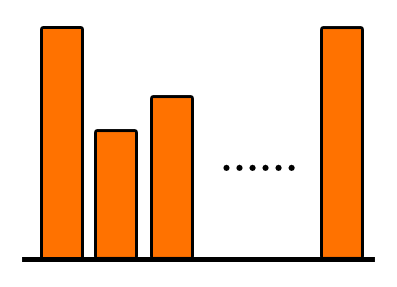
\includegraphics[width=5.00cm]{imgs/ch3/histogram}

\subsection{K近邻算法与相似性度量}
视觉词码表相当于将所有的特征向量分成若干类,每一类有类中心和类标号,下一节将讨论如何在广泛使用的K聚类算法上进行优化,利用相似K聚类进行快速的聚类来生成视觉词码表。本节探讨在视觉词码表存在的情况下,如何找到某一个特征向量对应的类。

确定空间中某个实例所属的类这一分类问题最常用的解决方案是K近邻算法。

K近邻算法(K-Nearest Neighbor algorithm,KNN)是给定一个训练数据集,对新的输入实例,在训练数据集中找到与该实例最邻近的K个实例,这K个实例的多数属于某个类,就把该输入实例分类到这个类中。

如何找到邻居,邻居的判定标准是什么,用什么来度量是本章探讨的主要问题。特征空间中两个实例点的距离反应出两个实例点之间的相似性程度。K近邻模型的特征空间一般是n维实数向量空间,使用的距离可以使欧式距离、曼哈顿距离、标准化欧氏距离、汉明距离、夹角余弦等,由于篇幅所限,这里不一一例举。

值得说明的是,当K为1的时候,K近邻算法自然的转化为最近邻算法。上一章中我们探讨了k-d树的使用,就是最近邻算法的加速算法之一,而下一节局部特征聚类中我们将探讨利用多颗k-d树组成森林的技术,对K近邻算法进行加速。

%[相似度计算](http://blog.sina.com.cn/s/blog_6634c1410100w56x.html)
%http://www.cnblogs.com/v-July-v/archive/2012/11/20/3125419.html

\subsection{局部特征的聚类}
生成视觉词码表是将局部特征进行聚类的过程,最经典的聚类算法是K均值聚类(K-MEANS),在实际中,我们通常在云端图像语料集中随机的选取一部分的特征,对这部分特征使用K-MEANS进行聚类,确定所有类中心后,再对语料集中的所有特征进行处理,找到每一个特征距离最近的类中心,完成对所有局部特征的量化。后续的请求图像在提取特征后按照同样的方式进行量化。

然而,在本文提出的系统中,图像局部特征数量极大(对于上百万图像素的图像来说,每幅图像的sift数量平均在3000以上,100K的图像集上,有300M以上个128D的特征),传统的K-MEANS不能满足我们的性能要求,最近的一些研究针对图像据图特征提出了许多快速聚类的方法,文献\cite{Philbin:2007fk,Muja:2009uv,Wang:2010vs}等提出了近似K聚类(Approximate K-MEANS,AKM)和结构化K聚类(Hierarchy K-MEANS,HKM)的方案。

近似K-MEANS是传统K-MEANS的一种替代,传统的K-MEANS的时间花销主要是在计算特征点最近邻的类中心上,每一次迭代,我们需要计算每一个特征点,计算它和每一个类中心的距离,所以每次迭代的时间复杂度是\(O(NK)\),其中N是特征点数量,K是类中心的数量。在改进的版本中,每一次迭代之前,我们使用随机k-d森林来构建类中心来加快速度。在常规的k-d树中,我们需要决定每一次划分是在哪一个维的哪一个点上,通常我们选择方差最大的一个维度作为划分维度,以该维度上中值点作为划分点,在同一维度上比划分点小的点落在k-d数当前节点的左侧,大的落在右侧。在随机k-d森林中,每一棵k-d树都是构建在所有的类中心上,不过在构建时采用划分策略有所不同,划分维度是方差较大的几个维度中随机选择的,划分点也是随机的在中值附近选择一个点。所有的k-d树组成了k-d森林,这个森林构建了一个互相交叠的特征划分空间。因为量化的存在,一个在划分边缘的特征很可能找到错误的最近邻类中心,而互相交叠的划分方式则大大减轻了这一影响,增强了高维计算的鲁棒性。k-d森林中的k-d树的数量与训练集的样本数量有关,样本较大时,应该增加k-d树的数量,提高分类的准确性。

计算一个特征点所属类的过程如下:
对随机森林中的每一棵树,递归的下滤到其叶子节点,计算它到可区分边界的距离,将所有的距离记录在一个优先队列中。迭代的选择最近的划分,持续的将隐藏节点加入到优先级队列中,当迭代次数达到指定数值的时候,搜索停止。

K-MEANS的时间复杂度是\(O(NK+N) = O(NK)\),AKM算法的时间复杂度是\(O(Nlog(K)\)。实验表明,AKM在大幅降低时间复杂度的同时,保证了正确率,与K-MEANS相比较,划分类不一致的情况出现概率小于百分之一,能够满足我们的相似搜索要求。

%--------------------------------------TO Do Here---------------------------%



%%%%----------------------------------------改进--------------------------------------------%%%%
\section{大规模相似搜索优化算法}

随着数据规模的不断扩大,大规模相似搜索算法在近年来快速发展,主要从提高搜索精度以及搜索效率两个方面着手,通过充分挖掘局部特征信息记忆引入外部相关信息扩大搜索词来提升搜索精度,通过局部敏感哈希等算法压缩数据维度,提高搜索效率\cite{POLICY:2013te}。

相关学者近期提出了不同场景下进行相似搜索的优化方案,文献\cite{Li:2013ks}通过视觉显著性(saliency)模型进行比较,消除背景中的噪声。这种方法使得索引和匹配都集中在显著性区域,更能够符合用户的预期。显著值和空间约束都能够被用来进行相似性度量,并且能够高效的进行二级索引,对于大规模的部分相似图像搜索非常有利,但是内存开销比较大。

文献\cite{Negrel:2013ur}描述了目前存在的各种视觉描述子的概况,介绍了相关的索引技术,包括哈希、词袋以及基于树的表示方法。引出内存开销问题并提出一种生成高度压缩签名(highly compact signatures)的方法,包括张量聚合,主成分分析(PCA),基于核的主成分分析(kernel PCA)等一些列算法。它改进了费舍尔向量(Fisher Vector)族 描述子,提高它的可区分性,以及特征签名的大小。

对于相似性视频搜索,它的特点是特征维数特别大,有研究提出了稀疏投影方式进行特征降维,并且使用数据挖掘的知识使用一些元数据(metadata)来共同进行搜索\cite{Wu:2013tb}。使用机器学习技术,学习稀疏投影矩阵(sparse projection matrices)。这种学习方法可以选择性的使用外部信息,比如WikiPedia上的知识和Google搜索结果中的摘要,创建一个语义相关的投影矩阵,生成一个压缩签名,以满足手机媒体检索的诸多限制。手机内存空间小,计算资源有限,传统的将高维特征映射到低维的投影矩阵在手机内存是放不下的。而我们的稀疏投影矩阵是能够在手机上使用的。

本文在大规模数据集上做局部区域的部分相似图像搜索,上文提到的近邻算法难以满足性能要求,我们需要对搜索算法在性能上进行优化。
而我们知道图像搜索的许多算法借鉴于文本搜索,在文本的去重算法中常见的有余弦夹角算法、欧式距离、Jaccard相似度、最长公共子串、编辑距离等,但是只适合于小数据集。

当文档集规模很大时,这种方法因为比较耗时而难以实用,考虑到文档集中和已知文档相似的目标文档数一般不多,对上述方法的一种改进方案是首先快速获取那些可能相似的文档,然后对这个集合中的每个候选文档,进行具体的相似度计算验证。其中快速获取候选集可以通过一种叫做局部敏感哈希(Locality-sensitive hashing,简称 LSH)的技术来实现。这种技巧同样可以用在图像搜索的性能提升上,下面我们介绍其在图像搜索上的应用。

\subsection{最小哈希降维}
最小哈希(min-hash)是局部敏感哈希的一种,它能有效的数据降维的方式,广泛应用在相似性查找领域的算法。

在生成视觉词带之后,比较两幅图像或者两篇文章的相似度问题转化为比较两个只包含0,1元素的集合的相似度,集合的相似度是Jaccard相似度。
\begin{equation}
JS(A,B)=\frac{|A\cap{B}|}{|A\cup{B}|}
\end{equation}
我们首先定义一组随机哈希函数\(f_j:\mathcal{V} \to R\),每一个哈希函数是独立的,将一个视觉词映射为一个实数。两个不同的视觉词\(X_a\)和\(X_b\),哈希函数需要满足两点:
\begin{equation}
f_j(X_a)\neq f_j(X_b)
\end{equation}
和
\begin{equation}
P(f_j(X_a)) < (P(f_j(X_b)) = 0.5
\end{equation}

注意到函数\(f_j\)能够反映出视觉词集合的一个顺序排列情况,我们定义最小哈希就是这个排列中排在最前面的视觉词,因此有
\begin{equation}
m(A_i,f_j)= arg\mathop {\min }\limits_{X \in A_i}f_j(X)
\end{equation}

根据上述定义,我们会发现以下这个事实:
\begin{equation}
Pr(m(A,f_j) = (B,f_j)) = \frac{|A\cap{B}|}{|A\cup{B}|} = sim_s(A,B)
\end{equation}

如果r是随机变量,当\(m(A,f_j) = (B,f_j)\)时值为1,其它情况下值为0的,那么r可认为是J(A,B)的无偏估计。因此我们可以使用最小哈希函数将一幅图片或者一篇文章转化为一个数(对该文章中的每一个单词id使用hash函数后得到一个新的id序列,这个序列中的第一个出现1的行号,就是最小哈希的值),当我们使用k个hash函数,得到k个值,将原本的高维向量映射到了低维。最小哈希在压缩原始集合的情况下,保证了集合的相似度没有被破坏。
文献\cite{Chum:2008jo}中提出将词频-逆文档频率(term frequency–inverse document frequency,简称TF-IDF)融合在传统的最小哈希算法中,实验表明能够提高搜索的准确率。

\subsection{局部敏感哈希缩小查找范围}

使用上一节提到的最小哈希对数据降维后,可以使用LSH缩小查找范围,其基本思路是将相似的集合聚集到一起,减小查找范围,避免比较不相似的集合。

对每一列C(即每个集合)我们都计算出了N行最小哈希的值,我们把这N个值均分成B组,每组包含相邻的\(R=frac{N}{B}\)行。对于每一列,把其每组的R个数都算一个哈希值出来,把此列的编号记录到哈希值对应的桶(Bucket)里面。如果两列被放到了同一个桶里,说明它们至少有一组(R个)数的哈希值相同,此时可认为它们有较大可能相似度较高,称为一对候选组合。最后在比较时只对落在同一个桶里的集合两两计算,而不是全部的两两比较。

%%%%----------------------------------------空间信息匹配搜索算法--------------------------------------------%%%%

\section{基于局部相关信息的相似图像搜索算法}

使用视觉词袋模型来表示图像并比较视觉词频向量之间的相似性的方式应用极为广泛,因其建模简单、泛化能力强。但词袋模型忽略了图像包含位置关系这一天然属性,有学者提出利用空间信息进行图像的搜索任务,进一步挖掘图像本身的信息\cite{Philbin:2007fk,Wu:2009bl,Zhou:2010tv,Zhou:2013jz,Xu:2013wc}。值得注意的是,利用图像特征位置关系提升了匹配精度的同时,也加大了算法的复杂度,在实际使用时应根据任务特点选择合适的算法,空间信息在本文的使用是为了进行精确的图像配准和相似图像搜索。

本节将探讨如何利用图像特征点之间的空间位置和尺度相关性来进行更为精确的相似图像搜索,主体的搜索流程如图\ref{fig:similar_flowchar}所示。

\begin{figure}
\centering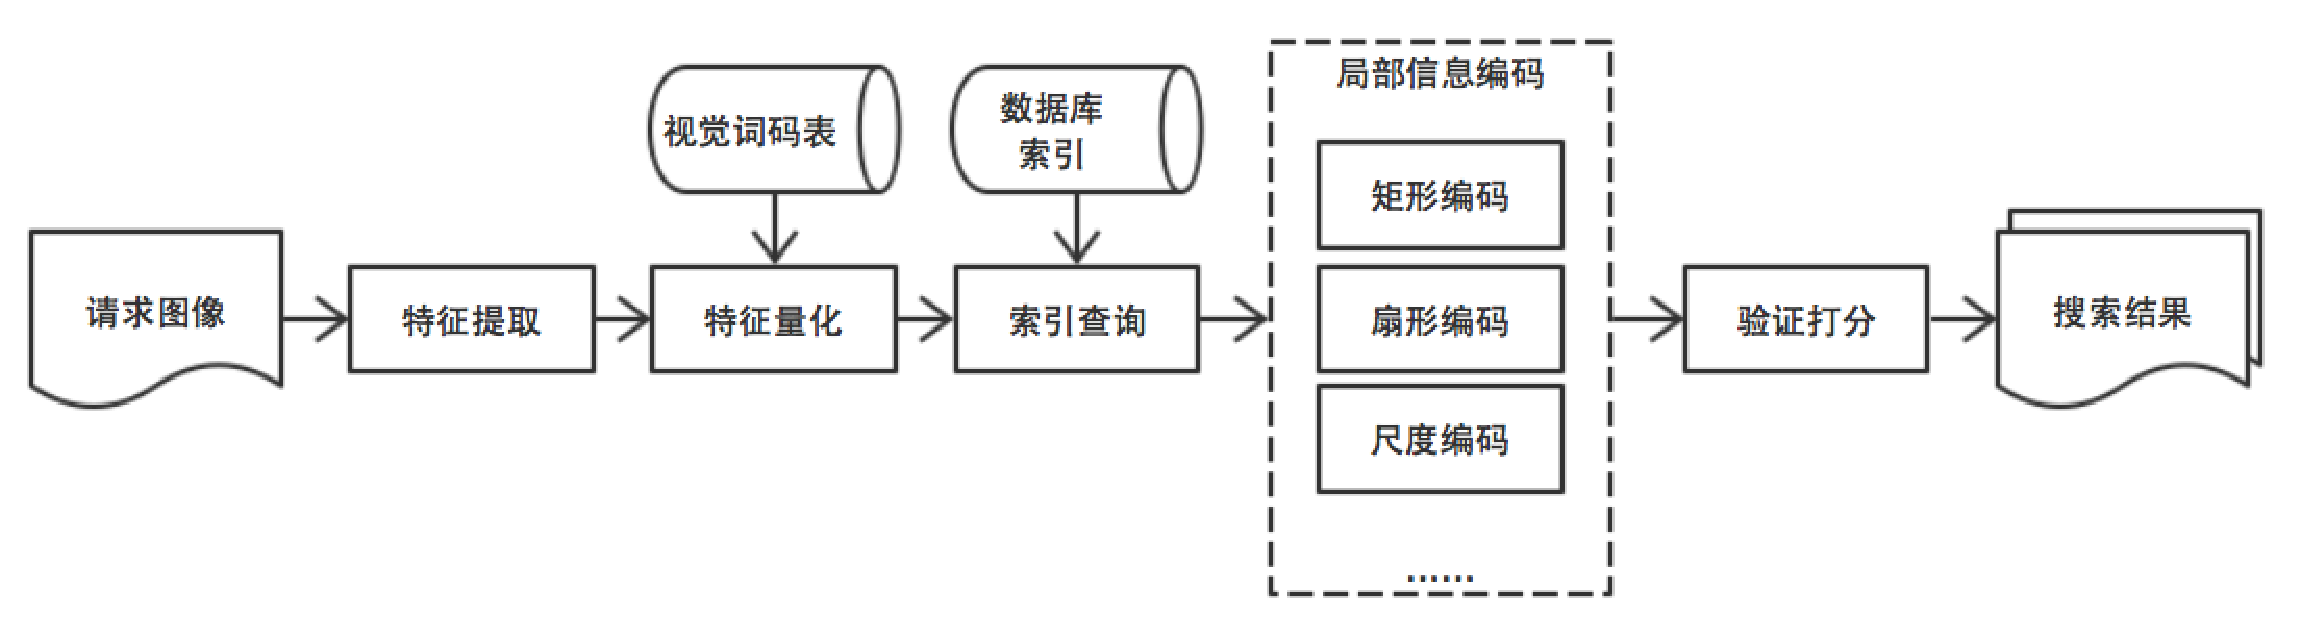
\includegraphics[width=16cm]{imgs/ch3/similar_flowchart}
\caption{利用局部相关信息进行图像搜索流程图}
\label{fig:similar_flowchar}
\end{figure}

其中虚线部分的编码方案有多种方式,可以单独使用,也可以混合使用。在实际中应根据应用具体场景采用不同的编码方案。

文献\cite{Xu:2013wc}深入研究SIFT描述子。提出了一个非常优雅的方法:生成SIFT组,嵌入几何信息,最终将一组SIFT压缩到一个64比特的二维签名中,叫做Nested-SIFT。Nested—SIFT使用SIFT描述子的嵌套关系,很自然的将不同尺度的局部关键点组合在一起,生成一个特征签名。嵌入空间信息的Nested—SIFT可区分性更强。使用SimHash进行压缩后,在视觉搜索中效率更高。实验结果表明这种方法提高搜索的准确度,减少了内存消耗,提高搜索速度。其缺点是生成Nested-SIFT会有一定的计算消耗。

文献\cite{Zhou:2013jz}采用较为复杂的空间编码,对图像2D空间进行了不同维度的划分,如图\ref{fig:geo_coding}所示。
\begin{figure}
\centering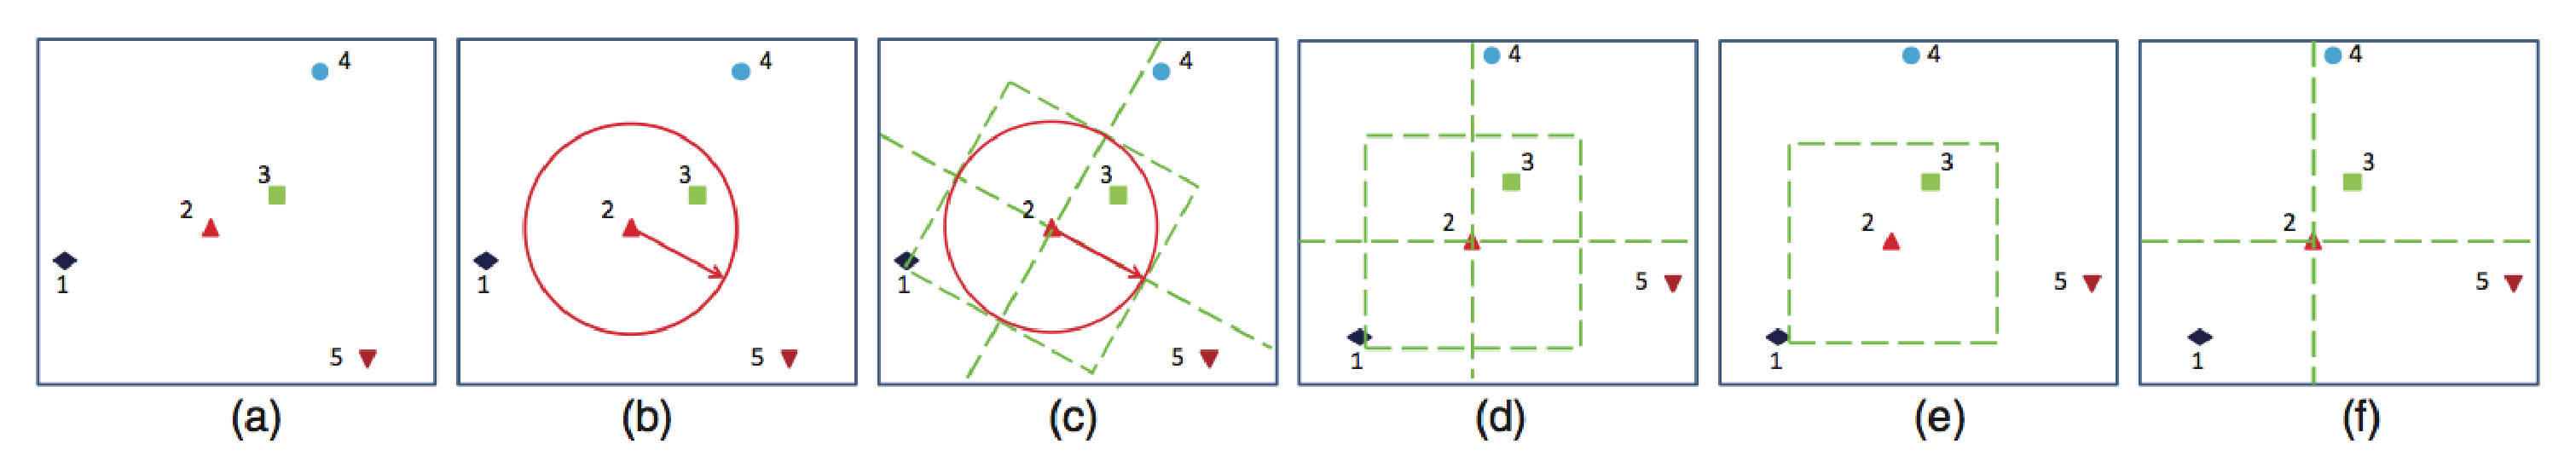
\includegraphics[width=15cm]{imgs/ch3/geo_coding}
\caption{几何编码示例图。(a)图像平面上的五个SIFT特征;(b)红色线条表示编号为2的SIFT特征的尺度、位置和方向;(c)图像平面分区(绿色线条表示);(d)根据c进行旋转后的结果;(e)和(f)表示两种不同的空间划分形式。}
\label{fig:geo_coding}
\end{figure}

首先从正方形区域区分了相邻特征是在区域内还是在区域外图(图\ref{fig:geo_coding}-(e)),其次加入了扇形区域的编码(图\ref{fig:geo_coding}-(f)),增加了视觉词组的旋转不变性。以两种空间划分方式生成编码结果,正如流程图\ref{fig:similar_flowchar}所示,将搜索的中间结果进行空间验证,去除不符合要求的中间结果。

实验结果表明加入空间信息验证后,能够提升准确率,两幅不相关的图像可能会有相似的特征集合,但是相似特征集合在空间位置上依然保持相似的概率极低。但该算法较为复杂,而且编码针对全局SIFT,更加适用于全局图像的相似查询而不适合本文的局部图像块的搜索。

因为本文系统需要查询的是具有局部相似的图像块,相比于其他相似性匹配算法,我们需要的图像块粒度更细,即云端图像与请求图像全局相似度可能很低,但是局部相似度非常高,这幅图像也会被加入到候选图像中。文献\cite{Dai:2012vn}提出了简洁的做法,将一个图像块内的局部特征编码成视觉词组。本文在该文基础上做了改进,在保证算法效率的同时,增加了对算子尺度的编码,进一步增强其准确度。

对于每一个图像块而言,中心位置有一个视觉词,该视觉词的尺度与其覆盖范围(影响范围)成正比,在该范围内,有若干视觉词,我们将范围内的所有视觉词看做一个视觉词组(Visual Words Group)。我们希望将词组内的每一个视觉词分配一个编码x,表征这个词在视觉词组的相对关系,这样我们可以采用如下的规则进行匹配:
\begin{equation}
E_m(G_x,G_y) = E_v(G_x,G_y) - E_r(G_x,G_y)
\end{equation}
其中\(E_v(G_x,G_y)\)是能够匹配上的视觉词,这里匹配上定义为两个视觉词相同,并且含有相同的编码x。其中\(E_r(G_x,G_y)\)是错误匹配的视觉词,错误匹配是指两个视觉词相同,但是含有不同的编码x。

那么怎样编码视觉词,能够体现视觉词的相对关系呢?我们从两个维度对视觉词进行编码,一个是它与中心视觉词的相对方向,另一个是相对尺度大小。视觉词组的中心词的主方向作为基准方向,沿着顺时针或者逆时针方向,将整个区域分成n个子区域。接下来对于每一个子区域,根据sift算子量化前的尺度信息对比值大小的不同,将子区域分成r个维度,这样一个视觉词共有n*r个子区域,如图\ref{fig:visual_group}所示。

\begin{figure}
\centering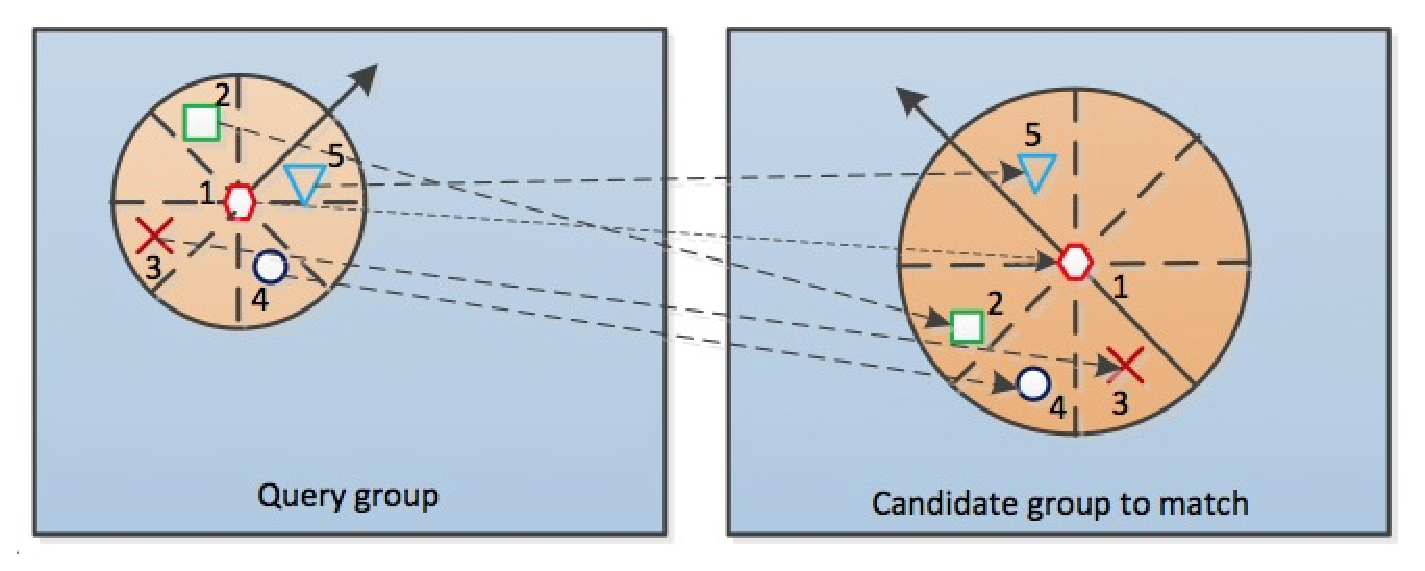
\includegraphics[width=15.00cm]{imgs/ch3/visual_group}
\caption{视觉词组二维编码}
\label{fig:visual_group}
\end{figure}

%%%%------------------------------------适用于旅游景点图像的相似图像搜索技术----------------------------------------%%%%
%\section{适用于旅游景点图像的相似图像搜索技术} 可以不提到

%% 本章参考文献
\ifx\usechapbib\empty
\nocite{BSTcontrol}
\bibliographystyle{buptgraduatethesis}
\bibliography{bare_thesis}
\fi